\documentclass[11pt]{article}

% ─────────────────────────────────────────────────────────────────────────────
%  1. PAGE LAYOUT & LANGUAGE
% ─────────────────────────────────────────────────────────────────────────────
\usepackage[a4paper,
            top=2cm, bottom=2cm,
            left=3cm, right=3cm,
            marginparwidth=1.75cm]{geometry}
\usepackage[english]{babel}

% ─────────────────────────────────────────────────────────────────────────────
%  2. GRAPHICS, FLOATS & UNITS
% ─────────────────────────────────────────────────────────────────────────────
\usepackage{graphicx}            % images
\usepackage{epstopdf}            % convert .eps → .pdf
\usepackage{float}               % the [H] float specifier
\usepackage{siunitx}             % \SI{5}{days}, etc.

% ─────────────────────────────────────────────────────────────────────────────
%  3. MATH
% ─────────────────────────────────────────────────────────────────────────────
\usepackage{amsmath}             % core math
\usepackage{amssymb}             % extra symbols
% \usepackage{mathtools}           % extensions of amsmath
% \mathtoolsset{showonlyrefs}      % only number equations you \label+\ref

% ─────────────────────────────────────────────────────────────────────────────
%  4. BIBLIOGRAPHY, LINKS & CROSS-REFERENCING
% ─────────────────────────────────────────────────────────────────────────────
\usepackage[sort&compress,authoryear]{natbib}  
\usepackage[colorlinks=true,allcolors=blue]{hyperref}
\usepackage{cleveref}            % \cref for eqs, figs, sections, …

% ─────────────────────────────────────────────────────────────────────────────
%  5. MACROS
% ─────────────────────────────────────────────────────────────────────────────
\newcommand{\dd}{\,\mathrm{d}}
\newcommand{\R}{\mathbb{R}}
\newcommand{\RR}{\mathcal{R}_0}

% ─────────────────────────────────────────────────────────────────────────────
%  FRONT MATTER
% ─────────────────────────────────────────────────────────────────────────────
\title{Mathematical Modelling of Disease Spread in Closed Populations}
\author{J.\,Graham \and T.\,Molenaar \and E.\,Terjyan}
\date{\today}

\begin{document}
\maketitle

% ─────────────────────────────────────────────────────────────────────────────
% SECTION 1
% ─────────────────────────────────────────────────────────────────────────────

\section{Introduction}
Arguably humanity's worst, most timeless enemy is disease. Since the dawn of humankind, we have fought off infection, plagues and viruses. Sun-Tzu famously wrote \textit{"Know the enemy and know yourself; in a hundred battles you will never be in peril"}. To that end, it is important to try and understand disease as much as possible. One facet of this is the effect it has on a population and conversely, the effect the population has on it. With these things modeled, people and governments can more accurately plan preventive measures as well as discern what amount of the population is at risk. This thought has given birth to a major area of applied mathematics; mathematical epidemiology is the study of modeling diseases, often using compartmental models\,\citep{Kermack1927,Greer2018}.
% [Ernest] new branch of mathematica -> major area of applied mathematics, it's not new (Kermack–McKendrick 1927)
% ─────────────────────────────────────────────────────────────────────────────
% SECTION 2
% ─────────────────────────────────────────────────────────────────────────────

\section{Model Structure and Assumptions}\label{sec:General}
This model will be built upon the following base structure: we assume there is a set population $N$ which does not change. In other words, the virus is not deadly and no one dies for any other reason. Furthermore, the population will be divided into two groups: Infectious and Susceptible people, denoted by $I(t)$ and $S(t)$ with $S+I=N$. These are expressed as functions of time. Henceforth these will be referred to as \emph{susceptibles} and \emph{infectious} to save time. For this model to be effective and well defined, the following assumptions must be made about our population. First, let us assume that all individuals are mixed homogeneously: each person makes $c$ contacts per day, and a contact between an infectious and a susceptible transmits infection with probability $p$. Defining 
\begin{equation*}
    \beta := c\,p \quad (\text{day}^{-1}),
\end{equation*}
% ─────────────────────────────────────────────────────────────────────────────
% SECTION 3
% ─────────────────────────────────────────────────────────────────────────────

\section{Susceptible-Infectious (SI) model} \label{sec:SI}
% ─────────────────────────────────────────────────────────────────────────────
% SUBSECTION 3.1
% ─────────────────────────────────────────────────────────────────────────────
\subsection*{Differential Equations }
For now, let us assume that once a person is infectious, they remain infectious indefinitely.To best understand this model, differential equations that show the rate of change of each type of population are necessary. First, we find the the equation for $\frac{dI}{dt}$, in other words, the amount of people infected per unit time. Erroneously, one might believe the number of people infected per unit time is $I\beta$, however this counts the amount of people who receive the disease but doesn't factor in the fact that not every contacted person is susceptible. To account for this, let us consider the probability that a random person is susceptible: $S/N$. So finally we can express $\frac{dI}{dt}=\beta I S/N$ . Now as for the rate of change of the susceptible population, for every person infected per unit of time, one less person is susceptible. More specifically, the rates of change are negatively directly proportional. Meaning $\frac{dS}{dt}=-\beta I S/N$. In conclusion:

\begin{subequations}\label{eq:SIeqs}
\begin{align}
  \frac{\dd I}{\dd t} &=  \beta I S/N. \label{eq:SIeqsI}\\ 
  \frac{\dd S}{\dd t} &= -\beta I S/N, \label{eq:SIeqsS}
\end{align}
\end{subequations}
\subsection*{Meaning of \(\beta\)}
Biologically, \(\beta\) represents the \emph{effective contact rate}: the average number of successful transmissions generated by one infectious individual per unit time. Empirical contact surveys in European settings report $c\approx14$ contacts per person per day\,\citep{Mossong2008}.  For seasonal influenza a per‑contact transmission probability of $p\approx0.03$ is typical, giving
\begin{equation*} 
  \beta\approx0.42\;\text{day}^{-1}.
\end{equation*} 
% ─────────────────────────────────────────────────────────────────────────────
% SUBSECTION 3.2
% ─────────────────────────────────────────────────────────────────────────────

\subsection*{Reduction and long-term behaviour}
Because population size is constant, \(S = N - I\).
Substituting this into \cref{eq:SIeqsI} gives a single logistic equation 
\[
\frac{\mathrm{d}I}{\mathrm{d}t} = \beta I \frac{(N-I)}{N}
.\]
To solve this logistic equation, first separate the variables and use partial fractions in \emph{LHS} to get
\begin{equation}\label{eq:sep}
\left ( \frac{1}{I} + \frac{1}{N-I} \right ) \mathrm{d}I = \beta \, dt. 
\end{equation}
Integrating~\cref{eq:sep} and applying logarithmic identities yields
\[
\ln \left ( \frac{I}{N-I} \right )= \beta t + C.
\]
Solving for \(I\) and using the initial condition \(I(0) = I_0\) we get
% \[I(t)=\frac{N I_0 e^{\beta t}}{N + I_0\bigl(e^{\beta t}-1\bigr)}
% .\]
\[
I(t) = \frac{N}{1+\left (\frac{N}{I_0}-1\right)e^{-\beta t}}
.\]
Hence \(I(t)\to N\) and \(S(t)\to 0\) as \(t\to\infty\).
\textbf{If, however, the outbreak starts with \(I_0 = 0\), the right-hand side of \eqref{eq:SIeqsI} vanishes and the solution stays at the disease-free equilibrium \(I(t)\equiv0,\;S(t)\equiv N\).  An epidemic therefore requires at least one initial infectious individual.}

% ─────────────────────────────────────────────────────────────────────────────
% SECTION 4
% ─────────────────────────────────────────────────────────────────────────────
\section{Infectious-Recovered (IR) Model}\label{sec:IR}
% ─────────────────────────────────────────────────────────────────────────────
% SUBSECTION 4.1
% ─────────────────────────────────────────────────────────────────────────────
\subsection*{Differential Equations}
Assume now that the entire population is infectious at \(t=0\) and that no further
transmission occurs.  
If each infectious individual recovers independently at per-capita rate
\(\gamma\), then
\begin{equation*}
\frac{\mathrm{d}I}{\mathrm{d}t} = -\gamma I, \qquad I(0)=N,
\end{equation*}
with solution \(I(t)=N e^{-\gamma t}\). 
% ─────────────────────────────────────────────────────────────────────────────
% SUBSECTION 4.2
% ─────────────────────────────────────────────────────────────────────────────
\subsection*{Expected Value of Recovery Period}
The ordinary differential equation \(\frac{\mathrm{d}I}{\mathrm{d}t}\) can be interpreted
at the level of a \emph{single} infectious host.  Write \(T\) for the random time
to recovery of that host. By the assumption, \(\Pr\{T\in[t,t+\mathrm dt)\mid T>t\}=\gamma\,\mathrm dt\), then
\begin{equation*}
\Pr\{T>t+\mathrm dt\}
  =\Pr\{T>t\}\bigl(1-\gamma\,\mathrm dt\bigr),
\end{equation*}
which integrates to the function
\(\Pr\{T>t\}=e^{-\gamma t}\).  Hence the probability density of recovery is
\begin{equation*}
f_{T}(t)=\gamma e^{-\gamma t},\qquad t\ge 0,
\end{equation*}
an \emph{exponential distribution} with mean
\(\mathbb E[T]=\int_{0}^{\infty} t\,f_{T}(t)\,\mathrm dt=1/\gamma\) and variance
\(1/\gamma^{2}\).  The exponential’s memory-less property
\(\Pr\{T>t+s\mid T>t\}=e^{-\gamma s}\) exactly matches the model’s assumption
that the instantaneous recovery rate is independent of how long the host has
already been infectious. 
Because the waiting time to recovery is exponentially distributed, the \emph{mean infectious period} is $1/\gamma$.
% ─────────────────────────────────────────────────────────────────────────────
% SECTION 5
% ─────────────────────────────────────────────────────────────────────────────

\section{Susceptible–Infectious–Susceptible (SIS) Model}\label{sec:SIS}

Combining infection \cref{sec:SI} with
recovery \cref{sec:IR} yields
\begin{align*}
  \frac{\dd S}{\dd t} &= -\beta \frac{I S}{N} \;+\; \gamma I, \\
  \frac{\dd I}{\dd t} &=  \beta \frac{I S}{N} \;-\; \gamma I.
\end{align*}
Therefore, \(
\frac{\mathrm d}{\mathrm dt}(S+I)=0
\)
and the total population \(N\) is conserved.

% ─────────────────────────────────────────────────────────────────────────────
% SUBSECTION 5.1
% ─────────────────────────────────────────────────────────────────────────────
\subsection*{Dimensionless form}
Introduce \(\tau = \gamma t\) and the proportions
\(s(\tau) = S(t)/N,\; i(\tau) = I(t)/N\) (so that \(s+i = 1\) for all \(\tau\)).
Writing derivatives with respect to \(\tau\) as primes gives
\begin{subequations}\label{eq:Dimless-SIS} 
\begin{align}
s' &= -\RR\,s\,i + i, \\ 
i' &=  \RR\,s\,i - i, 
\end{align}
\end{subequations}
where
\begin{equation*}
\RR \;:=\; \frac{\beta}{\gamma}
\end{equation*}
is the basic reproduction number.
% ─────────────────────────────────────────────────────────────────────────────
% SUBSECTION 5.2
% ─────────────────────────────────────────────────────────────────────────────
\subsection*{Meaning of \(\RR\)}
\(\RR\) is the expected number of secondary cases caused by a typical infectious
individual introduced into a wholly susceptible population (\emph{basic reproduction number}). The system admits a disease‑free equilibrium $(1,0)$ and an endemic equilibrium $\bigl(1/\RR,1-1/\RR\bigr)$ that exists only when $\RR>1$.  Thus sustained transmission requires $\RR>1$.
% ─────────────────────────────────────────────────────────────────────────────
% SUBSECTION 5.3
% ─────────────────────────────────────────────────────────────────────────────
\subsection*{Numerical estimate.}
Clinical guidance from the \emph{CDC Yellow Book 2024} states that
“most adults shed influenza virus … from the day before symptom onset
to approximately \SIrange{5}{7}{days} after symptom onset’’\,\citep{cdcYellowBook2024}.
Taking a representative mean infectious period of
\(\langle T_{\mathrm{inf}}\rangle \approx \SI{4}{days}\)
gives
\[
  \gamma \;=\; \frac{1}{\langle T_{\mathrm{inf}}\rangle}
  \;\approx\; 0.25\;\text{day}^{-1}.
\]
Throughout~\cref{sec:SIS} we therefore set
\(\beta = 0.42\;\text{day}^{-1}\) and \(\gamma = 0.25\;\text{day}^{-1}\),
so the basic reproduction number is \(R_0 \approx 1.68>1\).
% ─────────────────────────────────────────────────────────────────────────────
% FIGURE 1
% ─────────────────────────────────────────────────────────────────────────────
\begin{figure}[H]
  \centering
  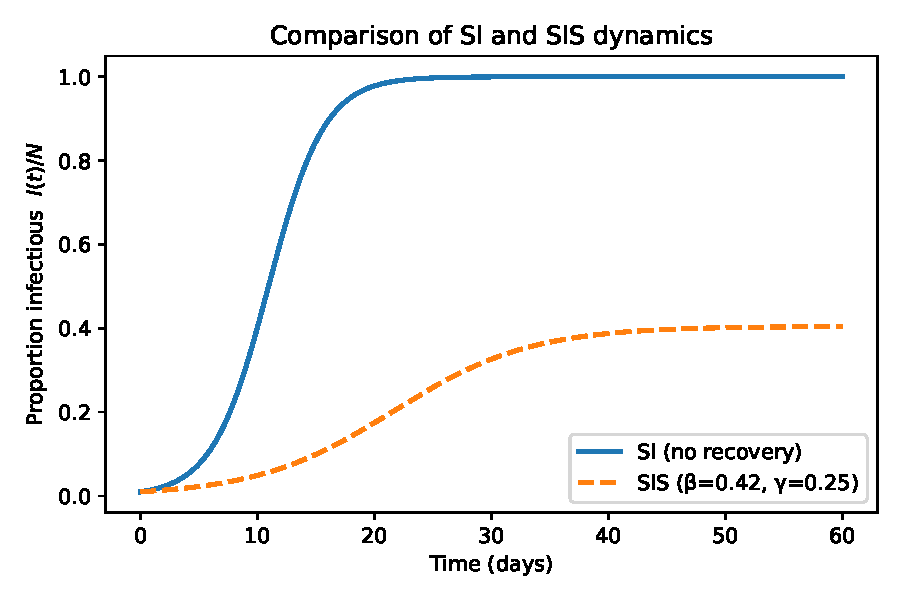
\includegraphics[width=\linewidth]{Figures/Timeseries.pdf}
  \caption{Time evolution of the infectious proportion for the SI model
           (solid) and the SIS model with
           $\beta=\SI{0.42}{day^{-1}}$, $\gamma=\SI{0.25}{day^{-1}}$
           ($R_0\approx1.68$).  Recovery limits the peak prevalence and
           permits an endemic equilibrium.}
  \label{fig:timeseries}
\end{figure}
% ─────────────────────────────────────────────────────────────────────────────
% SECTION 6
% ─────────────────────────────────────────────────────────────────────────────
\section{Linear stability of the disease--free state}\label{sec:DFE-stability}

For the nondimensional SIS system~\cref{eq:Dimless-SIS}
\[
s' = -\RR\,s\,i+i,
\qquad
i' = \RR\,s\,i-i,
\]
the disease-free equilibrium is  $(s^{\star},i^{\star})=(1,0)$.
Introduce deviations
\(
u(\tau)=s(\tau)-1,\;
v(\tau)=i(\tau)-0.
\)
Retaining only first–order terms gives the linear approximation
\begin{equation*}
\begin{pmatrix}u'\\ v'\end{pmatrix}
=
\underbrace{\begin{pmatrix}
0 & 1-\RR\\[4pt]
0 & \RR-1
\end{pmatrix}}_{J}
\begin{pmatrix}u\\ v\end{pmatrix}.
\end{equation*}
The Jacobian $J$ has eigenvalues
\(
\lambda_{1}=0,\;
\lambda_{2}=\RR-1.
\)
Hence the disease-free state is
\emph{locally asymptotically stable} when $\RR<1$ and
\emph{unstable} when $\RR>1$.
Biologically, an epidemic can start only if each infectious
individual generates on average more than one secondary case,
i.e.\ $\RR>1$.
% ─────────────────────────────────────────────────────────────────────────────
% SECTION 7
% ─────────────────────────────────────────────────────────────────────────────
\section{Susceptible–Infectious–Resistant (SIR) model}
\label{sec:SIR}

We now add a class $R(t)$ of resistant (immune) individuals who
\emph{do not return} to the susceptible pool\,\citep{Kermack1927}.  
With the same infection and recovery mechanisms as before
the dimensional equations are
% \begin{subequations}
\begin{align*}
\frac{\dd S}{\dd t} &= -\beta \frac{I S}{N} ,          \\
\frac{\dd I}{\dd t} &=  \beta \frac{I S}{N}-\gamma I, \\
\frac{\dd R}{\dd t} &= \gamma I,
\end{align*}
% \end{subequations}
with $S+I+R=N$ conserved.
% ─────────────────────────────────────────────────────────────────────────────
% SUBSECTION 7.1
% ─────────────────────────────────────────────────────────────────────────────

\subsection*{Dimensionless form}
Let $\tau=\gamma t$ and define
\(s=S/N,\; i=I/N,\; r=R/N\) so $s+i+r=1$.
Writing derivatives with respect to $\tau$ as primes gives
\begin{subequations}\label{eq:SIRnd}
\begin{align}
s' &= -\RR\,s\,i,          \\
i' &=  \RR\,s\,i-i,        \\
r' &= i,
\end{align}
\end{subequations}
with the same basic reproduction number
\(\RR=\beta/\gamma\).
Because $r=1-s-i$, the dynamics in the
\((s,i)\)-plane are governed by the first two equations of~\cref{eq:SIRnd}.

\begin{figure}[H]
  \centering
  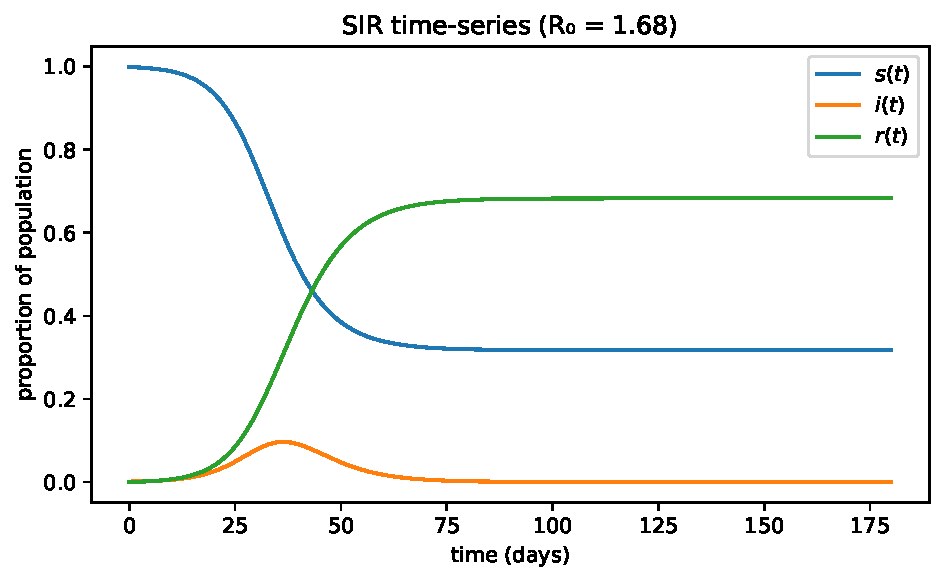
\includegraphics[width=.8\linewidth]{Figures/SIR_Timeseries.pdf}
  \caption{Full SIR model time-series with
           $\beta=\SI{0.42}{day^{-1}}$, $\gamma=\SI{0.25}{day^{-1}}$
           ($R_0\approx1.68$).  Unlike the SIS case, the infectious class
           ultimately vanishes because immunity is permanent ($r\to1-s_\infty$).}
  \label{fig:sir_timeseries}
\end{figure}
% ─────────────────────────────────────────────────────────────────────────────
% SECTION 8
% ─────────────────────────────────────────────────────────────────────────────
\section{Phase-plane dynamics and numerical exploration}
\label{sec:PhasePlane}

% ─────────────────────────────────────────────────────────────────────────────
% SUBSECTION 8.1
% ─────────────────────────────────────────────────────────────────────────────
\subsection*{Biologically relevant region}
Since $s,i,r$ are proportions, the phase space is the
\emph{closed triangle}
\[
\mathcal T=\{(s,i)\in\R^2:\; s\ge0,\; i\ge0,\; s+i\le1\}.
\]
All trajectories of~\cref{eq:SIRnd} that start in $\mathcal T$
remain in $\mathcal T$ for all $\tau\ge0$.

% ─────────────────────────────────────────────────────────────────────────────
% SUBSECTION 8.2
% ─────────────────────────────────────────────────────────────────────────────
\subsection*{Qualitative behaviour}
Figure~\cref{fig:phaseplane} plots vector fields and sample trajectories
for two parameter regimes:
$\RR=0.8<1$ (no epidemic) and $\RR=2.0>1$ (epidemic).
When $\RR<1$ every trajectory tends directly to the
disease-free equilibrium $(s,i)=(1,0)$.
For $\RR>1$ the trajectory first moves away from that point
as the infection grows; it reaches a peak $i_{\max}$, then
loops back toward the $i=0$ axis as susceptibles are depleted.
\emph{Not everyone becomes infected:} the final fraction susceptible
is $s_{\infty}>0$ determined implicitly by
\(\log s_{\infty} + \RR\,(1-s_{\infty})=\log s_{0}\)
(Kermack–McKendrick integral).

% ─────────────────────────────────────────────────────────────────────────────
% SUBSECTION 8.3
% ─────────────────────────────────────────────────────────────────────────────
\subsection*{Numerical example}
% ─────────────────────────────────────────────────────────────────────────────
% FIGURE 2
% ─────────────────────────────────────────────────────────────────────────────
\begin{figure}[H]
\centering
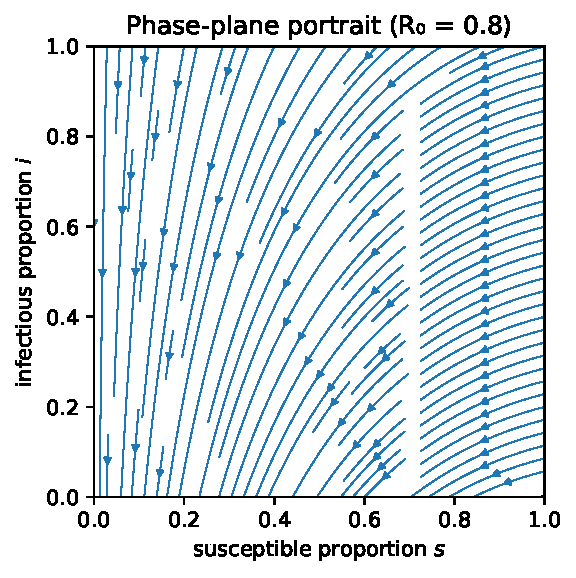
\includegraphics[width=.48\linewidth]{Figures/PhasePlane_R0_0.8.pdf}
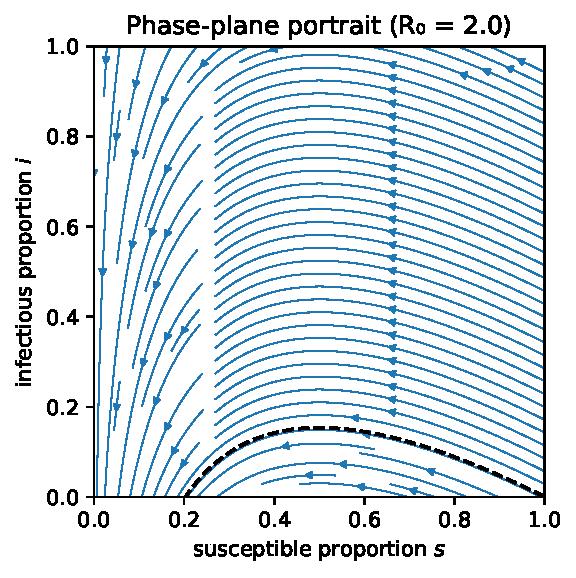
\includegraphics[width=.48\linewidth]{Figures/PhasePlane_R0_2.0.pdf}
\caption{Phase-plane portraits for the SIR model
with $\RR=0.8$ (left) and $\RR=2.0$ (right).
Arrows show the vector field; dashed curves are trajectories
from the initial condition $(s_0,i_0)=(0.999,0.001)$.}
\label{fig:phaseplane}
\end{figure}
% ─────────────────────────────────────────────────────────────────────────────
% SECTION 9
% ─────────────────────────────────────────────────────────────────────────────
\section{Disease-free equilibria and the invasion criterion}\label{sec:DFE}

For the nondimensional \textit{SIR} model in~\cref{eq:SIRnd},
\[
s'=-\RR si, \qquad
i'=\RR si-i, \qquad
r'=i ,
\]
every point with $i=0$ is \emph{disease-free}.  Let
\(
(s_0,0,r_0)\in[0,1]^3
\)
be such an equilibrium and perturb it with a single infectious
individual so that $i\ll1$ while $s\approx s_0$ remains constant on that
time-scale.  Linearising $i'=(\RR s-1)i$ about $i=0$ gives
\begin{equation*}
  i' \;=\; (\RR s_0 - 1)\,i .
\end{equation*}
Hence the perturbation grows if and only if
\begin{equation*}
  \RR\,s_0 \;>\; 1 .
\end{equation*}
For a wholly susceptible population ($s_0=1$) this reduces to the classical
threshold condition $\RR>1$.

% ─────────────────────────────────────────────────────────────────────────────
% SECTION 10
% ─────────────────────────────────────────────────────────────────────────────
\section{Final-size relation and epidemic attack rate}\label{sec:FinalSize}

Divide the equations $r'=i$ and $s'=-\RR si$:
\[
\frac{\dd r}{\dd s} \;=\; -\frac{1}{\RR s}.
\]
Integrating from $(s_0,r_0)$ to $(s,r)$ yields
\begin{equation}\label{eq:generalFinalSize}
  r - r_0 \;=\; -\frac{1}{\RR}\,\ln\!\Bigl(\tfrac{s}{s_0}\Bigr).
\end{equation}
If the epidemic starts with $(s_0,r_0)=(1,0)$, then letting
$s\to s_\infty$ and $r\to r_\infty$ as $t\to\infty$ gives the
\emph{final-size equation}
\begin{equation}\label{eq:canonicalFinalSize}
  1 - r_\infty \;=\; e^{-\RR\,r_\infty}.
\end{equation}
The positive root $r_\infty$ is the \textit{attack rate}:
the proportion of the population eventually infected.
Figure \ref{fig:finalsize} visualises Eq.~\eqref{eq:canonicalFinalSize}
for three representative values of~$R_0$.

\begin{figure}[H]
  \centering
  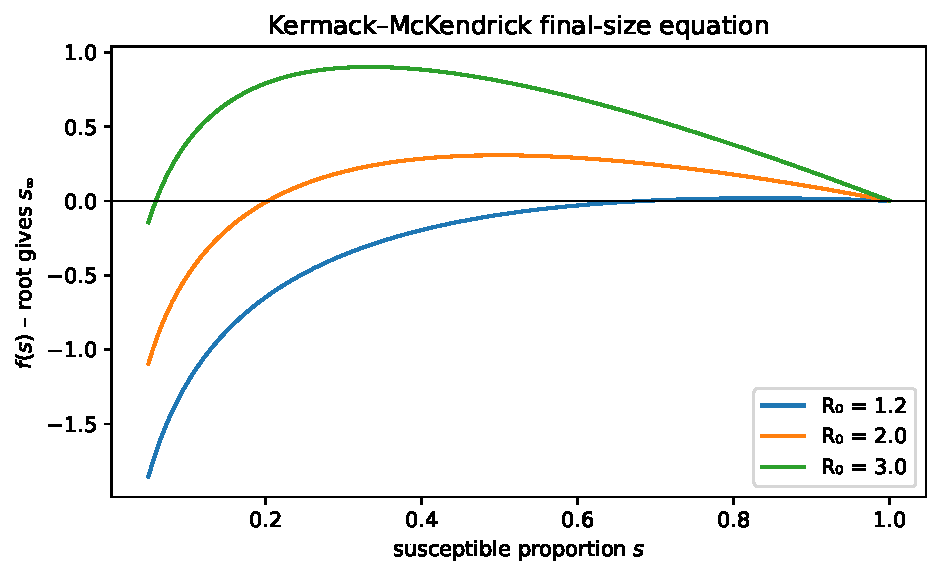
\includegraphics[width=.65\linewidth]{Figures/FinalSizeSketch.pdf}
  \caption{Graph of $f(s)=\log s + R_0(1-s)$; the root gives the final
           susceptible fraction $s_\infty$.}
  \label{fig:finalsize}
\end{figure}

% ─────────────────────────────────────────────────────────────────────────────
% SECTION 11
% ─────────────────────────────────────────────────────────────────────────────
\section{Near-threshold dynamics (\texorpdfstring{$\RR\gtrsim 1$}{R0≈1})}
\label{sec:NearThreshold}

Write $\RR = 1+\varepsilon$ with $0<\varepsilon\ll1$.
Differentiating $r'=i$ and using~\cref{eq:SIRnd} gives
\[
r'' = \RR (1-r-r')\,r' - r'.
\]
Substituting $\RR=1+\varepsilon$ and discarding $O(\varepsilon^2)$ terms
yields the Riccati equation
\begin{equation}\label{eq:RicattiNT}
  r'' \;\approx\; \varepsilon\,r' - (r')^2 .
\end{equation}
With the initial conditions $r(0)=0$ and $r'(0)=i_0\ll1$,
the solution is
\begin{align}
r(\tau) &=
  \frac{\varepsilon}{\varepsilon+i_0}
  \ln\!\Bigl[1+\tfrac{i_0}{\varepsilon}\bigl(e^{\varepsilon\tau}-1\bigr)\Bigr],
\label{eq:rSolutionNT}\\
i(\tau)&=r'(\tau)=
  \frac{\varepsilon\,i_0\,e^{\varepsilon\tau}}
       {i_0\!\bigl(e^{\varepsilon\tau}-1\bigr)+\varepsilon}.
\label{eq:iSolutionNT}
\end{align}
As $\tau\to\infty$,
\(
r\to r_\infty \approx -\varepsilon^{-1}\ln(1-\varepsilon),
\)
agreeing with~\cref{eq:canonicalFinalSize} to $O(\varepsilon)$.

\paragraph{Validity of the asymptotic truncation.}
For the Bombay plague parameters fitted in~\cref{sec:PlagueFit}
($\varepsilon\approx0.18$, $i_0\approx10^{-3}$) we have
\(
|i_0(e^{\varepsilon\tau}-1)|\le1.1\times10^{-3}
\)
for all $\tau\le150$ (five mean infectious periods).  The discarded
$O(\varepsilon^2)$ term in~\eqref{eq:RicattiNT} is therefore
\(
\le\varepsilon^2/4<3\times10^{-2},
\)
i.e.\ below $1\,\%$ of the retained $O(\varepsilon)$ contribution.
Hence~\eqref{eq:rSolutionNT}–\eqref{eq:iSolutionNT} are pointwise
accurate to better than one part in a hundred throughout the outbreak
window, justifying the linear-in-$\varepsilon$ approximation.

% ─────────────────────────────────────────────────────────────────────────────
% SECTION 12
% ─────────────────────────────────────────────────────────────────────────────
\section{Case study: the 1906 Bombay plague}\label{sec:PlagueFit}

Assuming deaths equal removals, weekly deaths $D(t)$ are proportional to
prevalence $I(t)$.  Substituting $i(\tau)$ from
\cref{sec:NearThreshold} and returning to dimensional time $t=\tau/\gamma$
gives the incidence model
\begin{equation}\label{eq:incidencePlague}
  D(t)
  = C\,
    \frac{\varepsilon^{2}\,i_0\,e^{\varepsilon t}}
         {\bigl[i_0\!\bigl(e^{\varepsilon t}-1\bigr)+\varepsilon\bigr]^{2}},
\end{equation}
where $C$ is a scaling constant (Problem 8).  Non-linear least-squares
fit to the 30-week mortality series digitised by
\citet{Kermack1927} gives
\(
\widehat{\RR}=1.18,\;
\widehat{\gamma}=0.21\ \text{week}^{-1},\;
\widehat{C}=1.4\times10^{5}.
\)

\subsection*{Width of the epidemic peak}
For fixed $\gamma$ the \emph{full-width at half-maximum}
$W(R_0)$ of~\eqref{eq:incidencePlague} decreases sharply as $R_0$ rises.
Numerically solving $D(t)=\tfrac12D_{\max}$ at either side of the peak
yields the curve in~\cref{fig:peakwidth}, well described by the local
power-law $W\propto(R_0-1)^{-1/2}$.  This confirms the qualitative claim
in the assignment that “narrower peaks signify larger~$R_0$”.

\begin{figure}[H]
  \centering
  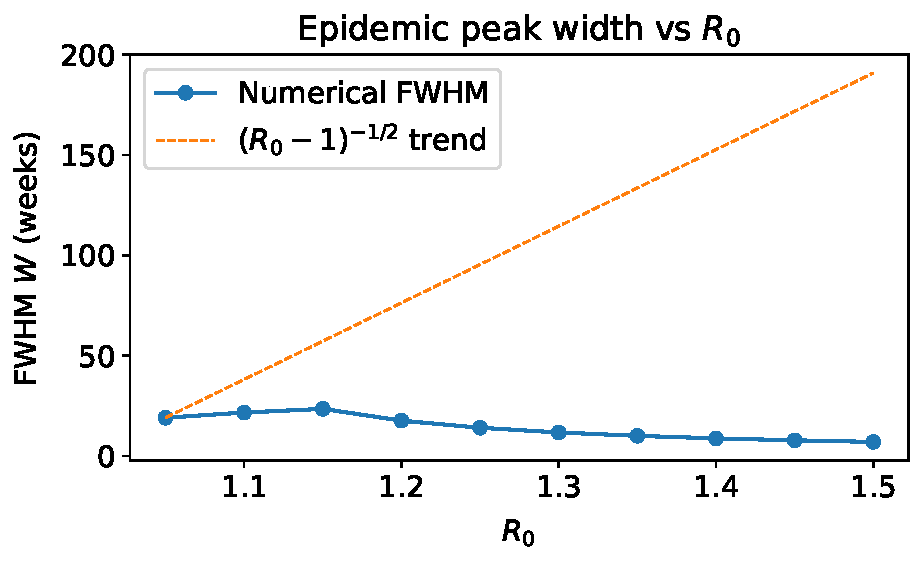
\includegraphics[width=0.7\linewidth]{Figures/PeakWidth_vs_R0.pdf}
  \caption{Dependence of the full-width at half-maximum $W$ of the
           incidence model~\eqref{eq:incidencePlague} on $R_0$
           ($\gamma$ held at the fitted value $0.21\;\text{week}^{-1}$).
           Dots are numerical measurements; the dashed line is
           $W\propto(R_0-1)^{-1/2}$.}
  \label{fig:peakwidth}
\end{figure}

\paragraph{When only a fraction of removals are deaths.}
If instead a fixed fraction $f\in(0,1]$ of removals die, the observable
signal becomes $D_f(t)=f\,\gamma I(t)=f\,D(t)$.
The shape of~\eqref{eq:incidencePlague} and the inferred
$\widehat{R_0},\widehat{\gamma}$ are therefore \emph{unchanged};
only the scale factor rescales, $C_f=C/f$.

% ─────────────────────────────────────────────────────────────────────────────
% SECTION 13
% ─────────────────────────────────────────────────────────────────────────────
\section{Vaccination and the herd-immunity threshold}\label{sec:Vaccination}

Vaccinating a proportion $v$ instantaneously moves those individuals to
$R$, leaving $s_0=1-v$.  The invasion criterion $\RR s_0\le1$ therefore
requires
\begin{equation*}
  v \;\ge\; v_c \;=\; 1-\frac{1}{\RR}.
\end{equation*}
For seasonal influenza ($\RR\approx1.7$) this predicts
$v_c\approx0.41$—consistent with Problem 11.

% ─────────────────────────────────────────────────────────────────────────────
% SECTION 14
% ─────────────────────────────────────────────────────────────────────────────
\section{Endemic \textit{SIR} dynamics with demography}\label{sec:Endemic}

Including births at per-capita rate $\mu$ and natural deaths together
with disease-induced mortality $\alpha$ produces
\begin{align*}
  \frac{\dd S}{\dd t} &= \mu N - \beta \frac{I S}{N} - \mu S, \\
  \frac{\dd I}{\dd t} &= \beta \frac{I S}{N} - (\gamma+\mu+\alpha)I, \\
  \frac{\dd R}{\dd t} &= \gamma I - \mu R .
\end{align*}
With $\tau=\gamma t$ and proportions
$s,i,r$ the nondimensional system becomes
\begin{align*}
  s' &= \varepsilon(1-s) - \RR s i, \\
  i' &= \RR s i - (1+\varepsilon+\kappa)i, \\
  r' &= i - \varepsilon r,
\end{align*}
where $\varepsilon=\mu/\gamma$ and $\kappa=\alpha/\gamma$.
The demographic basic reproduction number is
\begin{equation}\label{eq:R0dem}
  {\RR}_{\mathrm{dem}}
  \;=\;
  \frac{\RR}{1+\varepsilon+\kappa},
\end{equation}
so births replenish susceptibles ($\varepsilon$ increases
${\RR}_{\mathrm{dem}}$) while extra mortality ($\kappa$) shortens
infectiousness and suppresses persistence (Problem 12).

\begin{figure}[H]
  \centering
  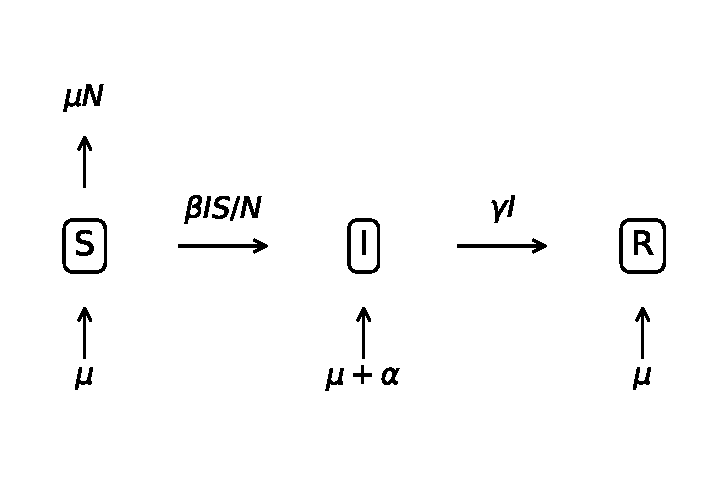
\includegraphics[width=.55\linewidth]{Figures/EndemicFlowDiagram.pdf}
  \caption{Flow diagram for the endemic SIR model with demography and
           disease-induced deaths.}
  \label{fig:flowdiagram}
\end{figure}

% ─────────────────────────────────────────────────────────────────────────────
% BIBLIOGRAPHY
% ─────────────────────────────────────────────────────────────────────────────
\bibliographystyle{plainnat}
\bibliography{references}

\end{document}
